% toolsoftrade/toolsoftrade.tex

\QuickQuizChapter{chp:Tools of the Trade}{Tools of the Trade}
%
\Epigraph{You are only as good as your tools, and your tools are only
	  as good as you are.}{\emph{Unknown}}

This chapter provides a brief introduction to some basic tools of the
parallel-programming trade, focusing mainly on those available to
user applications running on operating systems similar to Linux.
Section~\ref{sec:toolsoftrade:Scripting Languages} begins with
scripting languages,
Section~\ref{sec:toolsoftrade:POSIX Multiprocessing}
describes the multi-process parallelism supported by the POSIX API and
touches on POSIX threads,
@@@.
Section~\ref{sec:toolsoftrade:Linux-Kernel Equivalents to POSIX Operations}
presents the analogous operations within the Linux kernel, and finally,
Section~\ref{sec:toolsoftrade:The Right Tool for the Job: How to Choose?}
helps to choose the tool that will get the job done.

Please note that this chapter provides but a brief introduction.
More detail is available from the references cited, and more information
on how best to use these tools will be provided in later chapters.

\section{Scripting Languages}
\label{sec:toolsoftrade:Scripting Languages}

The Linux shell scripting languages provide simple but effective ways
of managing parallelism.
For example, suppose that you had a program \co{compute_it}
that you needed to run twice with two different sets of arguments.
This can be accomplished using UNIX shell scripting as follows:

\vspace{5pt}
\begin{minipage}[t]{\columnwidth}
\scriptsize
\begin{verbatim}
  1 compute_it 1 > compute_it.1.out &
  2 compute_it 2 > compute_it.2.out &
  3 wait
  4 cat compute_it.1.out
  5 cat compute_it.2.out
\end{verbatim}
\end{minipage}
\vspace{5pt}

\begin{figure}[tb]
\centering
\resizebox{3in}{!}{\includegraphics{toolsoftrade/shellparallel}}
\caption{Execution Diagram for Parallel Shell Execution}
\label{fig:intro:Execution Diagram for Parallel Shell Execution}
\end{figure}

Lines~1 and 2 launch two instances of this program, redirecting their
output to two separate files, with the \co{&} character directing the
shell to run the two instances of the program in the background.
Line~3 waits for both instances to complete, and lines~4 and 5
display their output.
The resulting execution is as shown in
Figure~\ref{fig:intro:Execution Diagram for Parallel Shell Execution}:
the two instances of \co{compute_it} execute in parallel,
\co{wait} completes after both of them do, and then the two instances
of \co{cat} execute sequentially.
% @@@ Maui scheduler, load balancing, BOINC, and so on.
% @@@ Diagram showing parallel execution.

\QuickQuiz{}
	But this silly shell script isn't a \emph{real} parallel program!
	Why bother with such trivia???
\QuickQuizAnswer{
	Because you should \emph{never} forget the simple stuff!

	Please keep in mind that the title of this book is
	``Is Parallel Programming Hard, And, If So, What Can You Do About It?''.
	One of the most effective things you can do about it is to
	avoid forgetting the simple stuff!
	After all, if you choose to do parallel programming the hard
	way, you have no one but yourself to blame.
} \QuickQuizEnd

\QuickQuiz{}
	Is there a simpler way to create a parallel shell script?
	If so, how?  If not, why not?
\QuickQuizAnswer{
	One straightforward approach is the shell pipeline:

\begin{minipage}[t]{\columnwidth}
\vspace{0.1ex}
\small
\begin{verbatim}
grep $pattern1 | sed -e 's/a/b/' | sort
\end{verbatim}
\vspace{0.1ex}
\end{minipage}

	For a sufficiently large input file,
	\co{grep} will pattern-match in parallel with \co{sed}
	editing and with the input processing of \co{sort}.
	See the file \co{parallel.sh} for a demonstration of
	shell-script parallelism and pipelining.
} \QuickQuizEnd

For another example, the \co{make} software-build scripting language
provides a \co{-j} option that specifies how much parallelism should be
introduced into the build process.
For example, typing \co{make -j4} when building a Linux kernel
specifies that up to four parallel compiles be carried out concurrently.

It is hoped that these simple examples convince you that parallel
programming need not always be complex or difficult.

\QuickQuiz{}
	But if script-based parallel programming is so easy, why
	bother with anything else?
\QuickQuizAnswer{
	In fact, it is quite likely that a very large fraction of
	parallel programs in use today are script-based.
	However, script-based parallelism does have its limitations:
	\begin{enumerate}
	\item	Creation of new processes is usually quite heavyweight,
		involving the expensive \co{fork()} and \co{exec()}
		system calls.
	\item	Sharing of data, including pipelining, typically involves
		expensive file I/O.
	\item	The reliable synchronization primitives available to
		scripts also typically involve expensive file I/O.
	\end{enumerate}
	These limitations require that script-based parallelism use
	coarse-grained parallelism, with each unit of work having
	execution time of at least tens of milliseconds, and preferably
	much longer.

	Those requiring finer-grained parallelism are well advised to
	think hard about their problem to see if it can be expressed
	in a coarse-grained form.
	If not, they should consider using other parallel-programming
	environments, such as those discussed in
	Section~\ref{sec:toolsoftrade:POSIX Multiprocessing}.
} \QuickQuizEnd

\section{POSIX Multiprocessing}
\label{sec:toolsoftrade:POSIX Multiprocessing}

This section scratches the surface of the
POSIX environment, including pthreads~\cite{OpenGroup1997pthreads},
as this environment is readily available and widely implemented.
Section~\ref{sec:toolsoftrade:POSIX Process Creation and Destruction}
provides a glimpse of the POSIX \co{fork()} and related primitives,
Section~\ref{sec:toolsoftrade:POSIX Thread Creation and Destruction}
touches on thread creation and destruction,
Section~\ref{sec:toolsoftrade:POSIX Locking} gives a brief overview
of POSIX locking, and, finally,
Section~\ref{sec:toolsoftrade:POSIX Reader-Writer Locking} describes a
specific lock which can be used for data that is read by many threads and only
occasionally updated.

\subsection{POSIX Process Creation and Destruction}
\label{sec:toolsoftrade:POSIX Process Creation and Destruction}

Processes are created using the \co{fork()} primitive, they may
be destroyed using the \co{kill()} primitive, they may destroy
themselves using the \co{exit()} primitive.
A process executing a \co{fork()} primitive is said to be the ``parent''
of the newly created process.
A parent may wait on its children using the \co{wait()} primitive.

Please note that the examples in this section are quite simple.
Real-world applications using these primitives might need to manipulate
signals, file descriptors, shared memory segments, and any number of
other resources.
In addition, some applications need to take specific actions if a given
child terminates, and might also need to be concerned with the reason
that the child terminated.
These concerns can of course add substantial complexity to the code.
For more information, see any of a number of textbooks on the
subject~\cite{WRichardStevens1992,StewartWeiss2013UNIX}.

\begin{figure}[tbp]
{ \scriptsize
\begin{verbbox}
  1 pid = fork();
  2 if (pid == 0) {
  3   /* child */
  4 } else if (pid < 0) {
  5   /* parent, upon error */
  6   perror("fork");
  7   exit(-1);
  8 } else {
  9   /* parent, pid == child ID */
 10 }
\end{verbbox}
}
\centering
\theverbbox
\caption{Using the fork() Primitive}
\label{fig:toolsoftrade:Using the fork() Primitive}
\end{figure}

If \co{fork()} succeeds, it returns twice, once for the parent
and again for the child.
The value returned from \co{fork()} allows the caller to tell
the difference, as shown in
Figure~\ref{fig:toolsoftrade:Using the fork() Primitive}
(\path{forkjoin.c}).
Line~1 executes the \co{fork()} primitive, and saves its return value
in local variable \co{pid}.
Line~2 checks to see if \co{pid} is zero, in which case, this is the
child, which continues on to execute line~3.
As noted earlier, the child may terminate via the \co{exit()} primitive.
Otherwise, this is the parent, which checks for an error return from
the \co{fork()} primitive on line~4, and prints an error and exits
on lines~5-7 if so.
Otherwise, the \co{fork()} has executed successfully, and the parent
therefore executes line~9 with the variable \co{pid} containing the
process ID of the child.

\begin{figure}[tbp]
{ \scriptsize
\begin{verbbox}
  1 void waitall(void)
  2 {
  3   int pid;
  4   int status;
  5 
  6   for (;;) {
  7     pid = wait(&status);
  8     if (pid == -1) {
  9       if (errno == ECHILD)
 10         break;
 11       perror("wait");
 12       exit(-1);
 13     }
 14   }
 15 }
\end{verbbox}
}
\centering
\theverbbox
\caption{Using the wait() Primitive}
\label{fig:toolsoftrade:Using the wait() Primitive}
\end{figure}

The parent process may use the \co{wait()} primitive to wait for its children
to complete.
However, use of this primitive is a bit more complicated than its shell-script
counterpart, as each invocation of \co{wait()} waits for but one child
process.
It is therefore customary to wrap \co{wait()} into a function similar
to the \co{waitall()} function shown in
Figure~\ref{fig:toolsoftrade:Using the wait() Primitive}
(\path{api-pthread.h}),
with this \co{waitall()} function having semantics similar to the
shell-script \co{wait} command.
Each pass through the loop spanning lines~6-15 waits on one child process.
Line~7 invokes the \co{wait()} primitive, which blocks until a child process
exits, and returns that child's process ID.
If the process ID is instead $-1$, this indicates that the \co{wait()}
primitive was unable to wait on a child.
If so, line~9 checks for the \co{ECHILD} errno, which indicates that there
are no more child processes, so that line~10 exits the loop.
Otherwise, lines~11 and 12 print an error and exit.

\QuickQuiz{}
	Why does this \co{wait()} primitive need to be so complicated?
	Why not just make it work like the shell-script \co{wait} does?
\QuickQuizAnswer{
	Some parallel applications need to take special action when
	specific children exit, and therefore need to wait for each
	child individually.
	In addition, some parallel applications need to detect the
	reason that the child died.
	As we saw in Figure~\ref{fig:toolsoftrade:Using the wait() Primitive},
	it is not hard to build a \co{waitall()} function out of
	the \co{wait()} function, but it would be impossible to
	do the reverse.
	Once the information about a specific child is lost, it is lost.
} \QuickQuizEnd

\begin{figure}[tbp]
{ \scriptsize
\begin{verbbox}
  1 int x = 0;
  2 int pid;
  3 
  4 pid = fork();
  5 if (pid == 0) { /* child */
  6   x = 1;
  7   printf("Child process set x=1\n");
  8   exit(0);
  9 }
 10 if (pid < 0) { /* parent, upon error */
 11   perror("fork");
 12   exit(-1);
 13 }
 14 waitall();
 15 printf("Parent process sees x=%d\n", x);
\end{verbbox}
}
\centering
\theverbbox
\caption{Processes Created Via fork() Do Not Share Memory}
\label{fig:toolsoftrade:Processes Created Via fork() Do Not Share Memory}
\end{figure}

It is critically important to note that the parent and child do \emph{not}
share memory.
This is illustrated by the program shown in
Figure~\ref{fig:toolsoftrade:Processes Created Via fork() Do Not Share Memory}
(\path{forkjoinvar.c}),
in which the child sets a global variable \co{x} to 1 on line~6,
prints a message on line~7, and exits on line~8.
The parent continues at line~14, where it waits on the child,
and on line~15 finds that its copy of the variable \co{x} is still zero.
The output is thus as follows:

\vspace{5pt}
\begin{minipage}[t]{\columnwidth}
\scriptsize
\begin{verbatim}
Child process set x=1
Parent process sees x=0
\end{verbatim}
\end{minipage}
\vspace{5pt}

\QuickQuiz{}
	Isn't there a lot more to \co{fork()} and \co{wait()}
	than discussed here?
\QuickQuizAnswer{
	Indeed there is, and
	it is quite possible that this section will be expanded in
	future versions to include messaging features (such as UNIX
	pipes, TCP/IP, and shared file I/O) and memory mapping
	(such as \co{mmap()} and \co{shmget()}).
	In the meantime, there are any number of textbooks that cover
	these primitives in great detail,
	and the truly motivated can read manpages, existing parallel
	applications using these primitives, as well as the
	source code of the Linux-kernel implementations themselves.

	It is important to note that the parent process in
	Figure~\ref{fig:toolsoftrade:Processes Created Via fork() Do Not Share Memory}
	waits until after the child terminates to do its \co{printf()}.
	Using \co{printf()}'s buffered I/O concurrently to the same file
	from multiple processes is non-trivial, and is best avoided.
	If you really need to do concurrent buffered I/O,
	consult the documentation for your OS.
	For UNIX/Linux systems, Stewart Weiss's lecture notes provide
	a good introduction with informative
	examples~\cite{StewartWeiss2013UNIX}.
} \QuickQuizEnd

The finest-grained parallelism requires shared memory, and
this is covered in
Section~\ref{sec:toolsoftrade:POSIX Thread Creation and Destruction}.
That said, shared-memory parallelism can be significantly more complex
than fork-join parallelism.

\subsection{POSIX Thread Creation and Destruction}
\label{sec:toolsoftrade:POSIX Thread Creation and Destruction}

To create a thread within an existing process, invoke the
\co{pthread_create()} primitive, for example, as shown on lines~15
and~16 of
Figure~\ref{fig:toolsoftrade:Threads Created Via pthread-create() Share Memory}
(\path{pcreate.c}).
The first argument is a pointer to a \co{pthread_t} in which to store the
ID of the thread to be created, the second \co{NULL} argument is a pointer
to an optional \co{pthread_attr_t}, the third argument is the function
(in this case, \co{mythread()})
that is to be invoked by the new thread, and the last \co{NULL} argument
is the argument that will be passed to \co{mythread}.

\begin{figure}[tbp]
{ \scriptsize
\begin{verbbox}
  1 int x = 0;
  2 
  3 void *mythread(void *arg)
  4 {
  5   x = 1;
  6   printf("Child process set x=1\n");
  7   return NULL;
  8 }
  9 
 10 int main(int argc, char *argv[])
 11 {
 12   pthread_t tid;
 13   void *vp;
 14 
 15   if (pthread_create(&tid, NULL,
 16                      mythread, NULL) != 0) {
 17     perror("pthread_create");
 18     exit(-1);
 19   }
 20   if (pthread_join(tid, &vp) != 0) {
 21     perror("pthread_join");
 22     exit(-1);
 23   }
 24   printf("Parent process sees x=%d\n", x);
 25   return 0;
 26 }
\end{verbbox}
}
\centering
\theverbbox
\caption{Threads Created Via {\tt pthread\_create()} Share Memory}
\label{fig:toolsoftrade:Threads Created Via pthread-create() Share Memory}
\end{figure}

In this example, \co{mythread()} simply returns, but it could instead
call \co{pthread_exit()}.

\QuickQuiz{}
	If the \co{mythread()} function in
	Figure~\ref{fig:toolsoftrade:Threads Created Via pthread-create() Share Memory}
	can simply return, why bother with \co{pthread_exit()}?
\QuickQuizAnswer{
	In this simple example, there is no reason whatsoever.
	However, imagine a more complex example, where \co{mythread()}
	invokes other functions, possibly separately compiled.
	In such a case, \co{pthread_exit()} allows these other functions
	to end the thread's execution without having to pass some sort
	of error return all the way back up to \co{mythread()}.
} \QuickQuizEnd

The \co{pthread_join()} primitive, shown on line~20,  is analogous to
the fork-join \co{wait()} primitive.
It blocks until the thread specified by the \co{tid} variable completes
execution, either by invoking \co{pthread_exit()} or by returning from
the thread's top-level function.
The thread's exit value will be stored through the pointer passed as the
second argument to \co{pthread_join()}.
The thread's exit value is either the value passed to \co{pthread_exit()}
or the value returned by the thread's top-level function, depending on
how the thread in question exits.

The program shown in
Figure~\ref{fig:toolsoftrade:Threads Created Via pthread-create() Share Memory}
produces output as follows, demonstrating that memory is in fact
shared between the two threads:

\vspace{5pt}
\begin{minipage}[t]{\columnwidth}
\scriptsize
\begin{verbatim}
Child process set x=1
Parent process sees x=1
\end{verbatim}
\end{minipage}
\vspace{5pt}

Note that this program carefully makes sure that only one of the threads
stores a value to variable \co{x} at a time.
Any situation in which one thread might be storing a value to a given
variable while some other thread either loads from or stores to that
same variable is termed a ``data race''.
Because the C language makes no guarantee that the results of a data race
will be in any way reasonable, we need some way of safely accessing
and modifying data concurrently, such as the locking primitives discussed
in the following section.

\QuickQuiz{}
	If the C language makes no guarantees in presence of a data
	race, then why does the Linux kernel have so many data races?
	Are you trying to tell me that the Linux kernel is completely
	broken???
\QuickQuizAnswer{
	Ah, but the Linux kernel is written in a carefully selected
	superset of the C language that includes special gcc
	extensions, such as asms, that permit safe execution even
	in presence of data races.
	In addition, the Linux kernel does not run on a number of
	platforms where data races would be especially problematic.
	For an example, consider embedded systems with 32-bit pointers
	and 16-bit busses.
	On such a system, a data race involving a store to and a load
	from a given pointer might well result in the load returning the
	low-order 16 bits of the old value of the pointer concatenated
	with the high-order 16 bits of the new value of the pointer.
} \QuickQuizEnd

\subsection{POSIX Locking}
\label{sec:toolsoftrade:POSIX Locking}

The POSIX standard allows the programmer to avoid data races via
``POSIX locking''.
POSIX locking features a number of primitives, the most fundamental
of which are \co{pthread_mutex_lock()} and \co{pthread_mutex_unlock()}.
These primitives operate on locks, which are of type \co{pthread_mutex_t}.
These locks may be declared statically and initialized with
\co{PTHREAD_MUTEX_INITIALIZER}, or they may be allocated dynamically
and initialized using the \co{pthread_mutex_init()} primitive.
The demonstration code in this section will take the former course.

The \co{pthread_mutex_lock()} primitive ``acquires'' the specified lock,
and the \co{pthread_mutex_unlock()} ``releases'' the specified lock.
Because these are ``exclusive'' locking primitives,
only one thread at a time may ``hold'' a given lock at a given time.
For example, if a pair of threads attempt to acquire the same lock
concurrently, one of the pair will be ``granted'' the lock first, and
the other will wait until the first thread releases the lock.

\QuickQuiz{}
	What if I want several threads to hold the same lock at the
	same time?
\QuickQuizAnswer{
	The first thing you should do is to ask yourself why you would
	want to do such a thing.
	If the answer is ``because I have a lot of data that is read
	by many threads, and only occasionally updated'', then
	POSIX reader-writer locks might be what you are looking for.
	These are introduced in
	Section~\ref{sec:toolsoftrade:POSIX Reader-Writer Locking}.

	Another way to get the effect of multiple threads holding
	the same lock is for one thread to acquire the lock, and
	then use \co{pthread_create()} to create the other threads.
	The question of why this would ever be a good idea is left
	to the reader.
} \QuickQuizEnd

\begin{figure}[tbp]
{ \scriptsize
\begin{verbbox}
  1 pthread_mutex_t lock_a = PTHREAD_MUTEX_INITIALIZER;
  2 pthread_mutex_t lock_b = PTHREAD_MUTEX_INITIALIZER;
  3 int x = 0;
  4 
  5 void *lock_reader(void *arg)
  6 {
  7   int i;
  8   int newx = -1;
  9   int oldx = -1;
 10   pthread_mutex_t *pmlp = (pthread_mutex_t *)arg;
 11 
 12   if (pthread_mutex_lock(pmlp) != 0) {
 13     perror("lock_reader:pthread_mutex_lock");
 14     exit(-1);
 15   }
 16   for (i = 0; i < 100; i++) {
 17     newx = ACCESS_ONCE(x);
 18     if (newx != oldx) {
 19       printf("lock_reader(): x = %d\n", newx);
 20     }
 21     oldx = newx;
 22     poll(NULL, 0, 1);
 23   }
 24   if (pthread_mutex_unlock(pmlp) != 0) {
 25     perror("lock_reader:pthread_mutex_unlock");
 26     exit(-1);
 27   }
 28   return NULL;
 29 }
 30 
 31 void *lock_writer(void *arg)
 32 {
 33   int i;
 34   pthread_mutex_t *pmlp = (pthread_mutex_t *)arg;
 35 
 36   if (pthread_mutex_lock(pmlp) != 0) {
 37     perror("lock_writer:pthread_mutex_lock");
 38     exit(-1);
 39   }
 40   for (i = 0; i < 3; i++) {
 41     ACCESS_ONCE(x)++;
 42     poll(NULL, 0, 5);
 43   }
 44   if (pthread_mutex_unlock(pmlp) != 0) {
 45     perror("lock_writer:pthread_mutex_unlock");
 46     exit(-1);
 47   }
 48   return NULL;
 49 }
\end{verbbox}
}
\centering
\theverbbox
\caption{Demonstration of Exclusive Locks}
\label{fig:toolsoftrade:Demonstration of Exclusive Locks}
\end{figure}

This exclusive-locking property is demonstrated using the code shown in
Figure~\ref{fig:toolsoftrade:Demonstration of Exclusive Locks}
(\path{lock.c}).
Line~1 defines and initializes a POSIX lock named \co{lock_a}, while
line~2 similarly defines and initializes a lock named \co{lock_b}.
Line~3 defines and initializes a shared variable ~\co{x}.

Lines~5-28 defines a function \co{lock_reader()} which repeatedly
reads the shared variable \co{x} while holding
the lock specified by \co{arg}.
Line~10 casts \co{arg} to a pointer to a \co{pthread_mutex_t}, as
required by the \co{pthread_mutex_lock()} and \co{pthread_mutex_unlock()}
primitives.

\QuickQuiz{}
	Why not simply make the argument to \co{lock_reader()}
	on line~5 of
	Figure~\ref{fig:toolsoftrade:Demonstration of Exclusive Locks}
	be a pointer to a \co{pthread_mutex_t}?
\QuickQuizAnswer{
	Because we will need to pass \co{lock_reader()} to
	\co{pthread_create()}.
	Although we could cast the function when passing it to
	\co{pthread_create()}, function casts are quite a bit
	uglier and harder to get right than are simple pointer casts.
} \QuickQuizEnd

Lines~12-15 acquire the specified \co{pthread_mutex_t}, checking
for errors and exiting the program if any occur.
Lines~16-23 repeatedly check the value of \co{x}, printing the new value
each time that it changes.
Line~22 sleeps for one millisecond, which allows this demonstration
to run nicely on a uniprocessor machine.
Lines~24-27 release the \co{pthread_mutex_t}, again checking for
errors and exiting the program if any occur.
Finally, line~28 returns \co{NULL}, again to match the function type
required by \co{pthread_create()}.

\QuickQuiz{}
	Writing four lines of code for each acquisition and release
	of a \co{pthread_mutex_t} sure seems painful!
	Isn't there a better way?
\QuickQuizAnswer{
	Indeed!
	And for that reason, the \co{pthread_mutex_lock()} and
	\co{pthread_mutex_unlock()} primitives are normally wrapped
	in functions that do this error checking.
	Later on, we will wrap them with the Linux kernel
	\co{spin_lock()} and \co{spin_unlock()} APIs.
} \QuickQuizEnd

Lines~31-49 of
Figure~\ref{fig:toolsoftrade:Demonstration of Exclusive Locks}
shows \co{lock_writer()}, which
periodically update the shared variable \co{x} while holding the
specified \co{pthread_mutex_t}.
As with \co{lock_reader()}, line~34 casts \co{arg} to a pointer
to \co{pthread_mutex_t}, lines~36-39 acquires the specified lock,
and lines~44-47 releases it.
While holding the lock, lines~40-43 increment the shared variable \co{x},
sleeping for five milliseconds between each increment.
Finally, lines~44-47 release the lock.

\begin{figure}[tbp]
{ \scriptsize
\begin{verbbox}
  1   printf("Creating two threads using same lock:\n");
  2   if (pthread_create(&tid1, NULL,
  3                      lock_reader, &lock_a) != 0) {
  4     perror("pthread_create");
  5     exit(-1);
  6   }
  7   if (pthread_create(&tid2, NULL,
  8                      lock_writer, &lock_a) != 0) {
  9     perror("pthread_create");
 10     exit(-1);
 11   }
 12   if (pthread_join(tid1, &vp) != 0) {
 13     perror("pthread_join");
 14     exit(-1);
 15   }
 16   if (pthread_join(tid2, &vp) != 0) {
 17     perror("pthread_join");
 18     exit(-1);
 19   }
\end{verbbox}
}
\centering
\theverbbox
\caption{Demonstration of Same Exclusive Lock}
\label{fig:toolsoftrade:Demonstration of Same Exclusive Lock}
\end{figure}

Figure~\ref{fig:toolsoftrade:Demonstration of Same Exclusive Lock}
shows a code fragment that runs \co{lock_reader()} and
\co{lock_writer()} as threads using the same lock, namely, \co{lock_a}.
Lines~2-6 create a thread running \co{lock_reader()}, and then
Lines~7-11 create a thread running \co{lock_writer()}.
Lines~12-19 wait for both threads to complete.
The output of this code fragment is as follows:

\vspace{5pt}
\begin{minipage}[t]{\columnwidth}
\scriptsize
\begin{verbatim}
Creating two threads using same lock:
lock_reader(): x = 0
\end{verbatim}
\end{minipage}
\vspace{5pt}

Because both threads are using the same lock, the \co{lock_reader()}
thread cannot see any of the intermediate values of \co{x} produced
by \co{lock_writer()} while holding the lock.

\QuickQuiz{}
	Is ``x = 0'' the only possible output from the code fragment
	shown in
	Figure~\ref{fig:toolsoftrade:Demonstration of Same Exclusive Lock}?
	If so, why?
	If not, what other output could appear, and why?
\QuickQuizAnswer{
	No.
	The reason that ``x = 0'' was output was that \co{lock_reader()}
	acquired the lock first.
	Had \co{lock_writer()} instead acquired the lock first, then
	the output would have been ``x = 3''.
	However, because the code fragment started \co{lock_reader()} first
	and because this run was performed on a multiprocessor,
	one would normally expect \co{lock_reader()} to acquire the
	lock first.
	However, there are no guarantees, especially on a busy system.
} \QuickQuizEnd

\begin{figure}[tbp]
{ \scriptsize
\begin{verbbox}
  1   printf("Creating two threads w/different locks:\n");
  2   x = 0;
  3   if (pthread_create(&tid1, NULL,
  4                      lock_reader, &lock_a) != 0) {
  5     perror("pthread_create");
  6     exit(-1);
  7   }
  8   if (pthread_create(&tid2, NULL,
  9                      lock_writer, &lock_b) != 0) {
 10     perror("pthread_create");
 11     exit(-1);
 12   }
 13   if (pthread_join(tid1, &vp) != 0) {
 14     perror("pthread_join");
 15     exit(-1);
 16   }
 17   if (pthread_join(tid2, &vp) != 0) {
 18     perror("pthread_join");
 19     exit(-1);
 20   }
\end{verbbox}
}
\centering
\theverbbox
\caption{Demonstration of Different Exclusive Locks}
\label{fig:toolsoftrade:Demonstration of Different Exclusive Locks}
\end{figure}

Figure~\ref{fig:toolsoftrade:Demonstration of Different Exclusive Locks}
shows a similar code fragment, but this time using different locks:
\co{lock_a} for \co{lock_reader()} and \co{lock_b} for
\co{lock_writer()}.
The output of this code fragment is as follows:

\vspace{5pt}
\begin{minipage}[t]{\columnwidth}
\scriptsize
\begin{verbatim}
Creating two threads w/different locks:
lock_reader(): x = 0
lock_reader(): x = 1
lock_reader(): x = 2
lock_reader(): x = 3
\end{verbatim}
\end{minipage}
\vspace{5pt}

Because the two threads are using different locks, they do not exclude
each other, and can run concurrently.
The \co{lock_reader()} function can therefore see the intermediate
values of \co{x} stored by \co{lock_writer()}.

\QuickQuiz{}
	Using different locks could cause quite a bit of confusion,
	what with threads seeing each others' intermediate states.
	So should well-written parallel programs restrict themselves
	to using a single lock in order to avoid this kind of confusion?
\QuickQuizAnswer{
	Although it is sometimes possible to write a program using a
	single global lock that both performs and scales well, such
	programs are exceptions to the rule.
	You will normally need to use multiple locks to attain good
	performance and scalability.

	One possible exception to this rule is ``transactional memory'',
	which is currently a research topic.
	Transactional\-/memory semantics can be loosely thought of as those
	of a single global lock with optimizations permitted and
	with the addition of rollback~\cite{HansJBoehm2009HOTPAR}.
} \QuickQuizEnd

\QuickQuiz{}
	In the code shown in
	Figure~\ref{fig:toolsoftrade:Demonstration of Different Exclusive Locks},
	is \co{lock_reader()} guaranteed to see all the values produced
	by \co{lock_writer()}?
	Why or why not?
\QuickQuizAnswer{
	No.
	On a busy system, \co{lock_reader()} might be preempted
	for the entire duration of \co{lock_writer()}'s execution,
	in which case it would not see \emph{any} of \co{lock_writer()}'s
	intermediate states for \co{x}.
} \QuickQuizEnd

\QuickQuiz{}
	Wait a minute here!!!
	Figure~\ref{fig:toolsoftrade:Demonstration of Same Exclusive Lock}
	didn't initialize shared variable \co{x},
	so why does it need to be initialized in
	Figure~\ref{fig:toolsoftrade:Demonstration of Different Exclusive Locks}?
\QuickQuizAnswer{
	See line~3 of
	Figure~\ref{fig:toolsoftrade:Demonstration of Exclusive Locks}.
	Because the code in
	Figure~\ref{fig:toolsoftrade:Demonstration of Same Exclusive Lock}
	ran first, it could rely on the compile-time initialization of
	\co{x}.
	The code in
	Figure~\ref{fig:toolsoftrade:Demonstration of Different Exclusive Locks}
	ran next, so it had to re-initialize \co{x}.
} \QuickQuizEnd

Although there is quite a bit more to POSIX exclusive locking, these
primitives provide a good start and are in fact sufficient in a great
many situations.
The next section takes a brief look at POSIX reader-writer locking.

\subsection{POSIX Reader-Writer Locking}
\label{sec:toolsoftrade:POSIX Reader-Writer Locking}

The POSIX API provides a reader-writer lock, which is represented by
a \co{pthread_rwlock_t}.
As with \co{pthread_mutex_t}, \co{pthread_rwlock_t} may be statically
initialized via \co{PTHREAD_RWLOCK_INITIALIZER} or dynamically
initialized via the \co{pthread_rwlock_init()} primitive.
The \co{pthread_rwlock_rdlock()} primitive read-acquires the
specified \co{pthread_rwlock_t}, the \co{pthread_rwlock_wrlock()}
primitive write-acquires it, and the \co{pthread_rwlock_unlock()}
primitive releases it.
Only a single thread may write-hold a given \co{pthread_rwlock_t}
at any given time, but multiple threads may read-hold a given
\co{pthread_rwlock_t}, at least while there is no thread
currently write-holding it.

As you might expect, reader-writer locks are designed for read-mostly
situations.
In these situations, a reader-writer lock can provide greater scalability
than can an exclusive lock because the exclusive lock is by definition
limited to a single thread holding the lock at any given time, while
the reader-writer lock permits
an arbitrarily large number of readers to concurrently hold the lock.
However, in practice, we need to know how much additional scalability is
provided by reader-writer locks.

\begin{figure}[tbp]
{ \scriptsize
\begin{verbbox}
  1 pthread_rwlock_t rwl = PTHREAD_RWLOCK_INITIALIZER;
  2 int holdtime = 0;
  3 int thinktime = 0;
  4 long long *readcounts;
  5 int nreadersrunning = 0;
  6 
  7 #define GOFLAG_INIT 0
  8 #define GOFLAG_RUN  1
  9 #define GOFLAG_STOP 2
 10 char goflag = GOFLAG_INIT;
 11 
 12 void *reader(void *arg)
 13 {
 14   int i;
 15   long long loopcnt = 0;
 16   long me = (long)arg;
 17 
 18   __sync_fetch_and_add(&nreadersrunning, 1);
 19   while (ACCESS_ONCE(goflag) == GOFLAG_INIT) {
 20     continue;
 21   }
 22   while (ACCESS_ONCE(goflag) == GOFLAG_RUN) {
 23     if (pthread_rwlock_rdlock(&rwl) != 0) {
 24       perror("pthread_rwlock_rdlock");
 25       exit(-1);
 26     }
 27     for (i = 1; i < holdtime; i++) {
 28       barrier();
 29     }
 30     if (pthread_rwlock_unlock(&rwl) != 0) {
 31       perror("pthread_rwlock_unlock");
 32       exit(-1);
 33     }
 34     for (i = 1; i < thinktime; i++) {
 35       barrier();
 36     }
 37     loopcnt++;
 38   }
 39   readcounts[me] = loopcnt;
 40   return NULL;
 41 }
\end{verbbox}
}
\centering
\theverbbox
\caption{Measuring Reader-Writer Lock Scalability}
\label{fig:toolsoftrade:Measuring Reader-Writer Lock Scalability}
\end{figure}

Figure~\ref{fig:toolsoftrade:Measuring Reader-Writer Lock Scalability}
(\path{rwlockscale.c})
shows one way of measuring reader-writer lock scalability.
Line~1 shows the definition and initialization of the reader-writer
lock, line~2 shows the \co{holdtime} argument controlling the
time each thread holds the reader-writer lock,
line~3 shows the \co{thinktime} argument controlling the time between
the release of the reader-writer lock and the next acquisition,
line~4 defines the \co{readcounts} array into which each reader thread
places the number of times it acquired the lock, and
line~5 defines the \co{nreadersrunning} variable, which
determines when all reader threads have started running.

Lines~7-10 define \co{goflag}, which synchronizes the start and the
end of the test.
This variable is initially set to \co{GOFLAG_INIT}, then set to
\co{GOFLAG_RUN} after all the reader threads have started, and finally
set to \co{GOFLAG_STOP} to terminate the test run.

Lines~12-41 define \co{reader()}, which is the reader thread.
Line~18 atomically increments the \co{nreadersrunning} variable
to indicate that this thread is now running, and
lines~19-21 wait for the test to start.
The \co{ACCESS_ONCE()} primitive forces the compiler to fetch \co{goflag}
on each pass through the loop---the compiler would otherwise be within its
rights to assume that the value of \co{goflag} would never change.

\QuickQuiz{}
	Instead of using \co{ACCESS_ONCE()} everywhere, why not just
	declare \co{goflag} as \co{volatile} on line~10 of
	Figure~\ref{fig:toolsoftrade:Measuring Reader-Writer Lock Scalability}?
\QuickQuizAnswer{
	A \co{volatile} declaration is in fact a reasonable alternative in
	this particular case.
	However, use of \co{ACCESS_ONCE()} has the benefit of clearly
	flagging to the reader that \co{goflag} is subject to concurrent
	reads and updates.
	However, \co{ACCESS_ONCE()} is especially useful in cases where
	most of the accesses are protected by a lock (and thus \emph{not}
	subject to change), but where a few of the accesses are made outside
	of the lock.
	Using a volatile declaration in this case would make it harder
	for the reader to note the special accesses outside of the lock,
	and would also make it harder for the compiler to generate good
	code under the lock.
} \QuickQuizEnd

\QuickQuiz{}
	\co{ACCESS_ONCE()} only affects the compiler, not the CPU.
	Don't we also need memory barriers to make sure
	that the change in \co{goflag}'s value propagates to the
	CPU in a timely fashion in
	Figure~\ref{fig:toolsoftrade:Measuring Reader-Writer Lock Scalability}?
\QuickQuizAnswer{
	No, memory barriers are not needed and won't help here.
	Memory barriers only enforce ordering among multiple
	memory references:  They do absolutely nothing to expedite
	the propagation of data from one part of the system to
	another.
	This leads to a quick rule of thumb:  You do not need
	memory barriers unless you are using more than one
	variable to communicate between multiple threads.

	But what about \co{nreadersrunning}?
	Isn't that a second variable used for communication?
	Indeed it is, and there really are the needed memory-barrier
	instructions buried in \co{__sync_fetch_and_add()},
	which make sure that the thread proclaims its presence
	before checking to see if it should start.
} \QuickQuizEnd

\QuickQuiz{}
	Would it ever be necessary to use \co{ACCESS_ONCE()} when accessing
	a per-thread variable, for example, a variable declared using
	the \co{gcc} \co{__thread} storage class?
\QuickQuizAnswer{
	It depends.
	If the per-thread variable was accessed only from its thread,
	and never from a signal handler, then no.
	Otherwise, it is quite possible that \co{ACCESS_ONCE()} is needed.
	We will see examples of both situations in
	Section~\ref{sec:count:Signal-Theft Limit Counter Implementation}.

	This leads to the question of how one thread can gain access to
	another thread's \co{__thread} variable, and the answer is that
	the second thread must store a pointer to its \co{__thread}
	pointer somewhere that the first thread has access to.
	One common approach is to maintain a linked list with one 
	element per thread, and to store the address of each thread's
	\co{__thread} variable in the corresponding element.
} \QuickQuizEnd

The loop spanning lines~22-38 carries out the performance test.
Lines~23-26 acquire the lock, lines~27-29 hold the lock for the specified
duration (and the \co{barrier()} directive prevents the compiler from
optimizing the loop out of existence), lines~30-33 release the lock,
and lines~34-36 wait for the specified duration before re-acquiring the
lock.
Line~37 counts this lock acquisition.

Line~39 moves the lock-acquisition count to this thread's element of the
\co{readcounts[]} array, and line~40 returns, terminating this thread.

\begin{figure}[tb]
\centering
\resizebox{3in}{!}{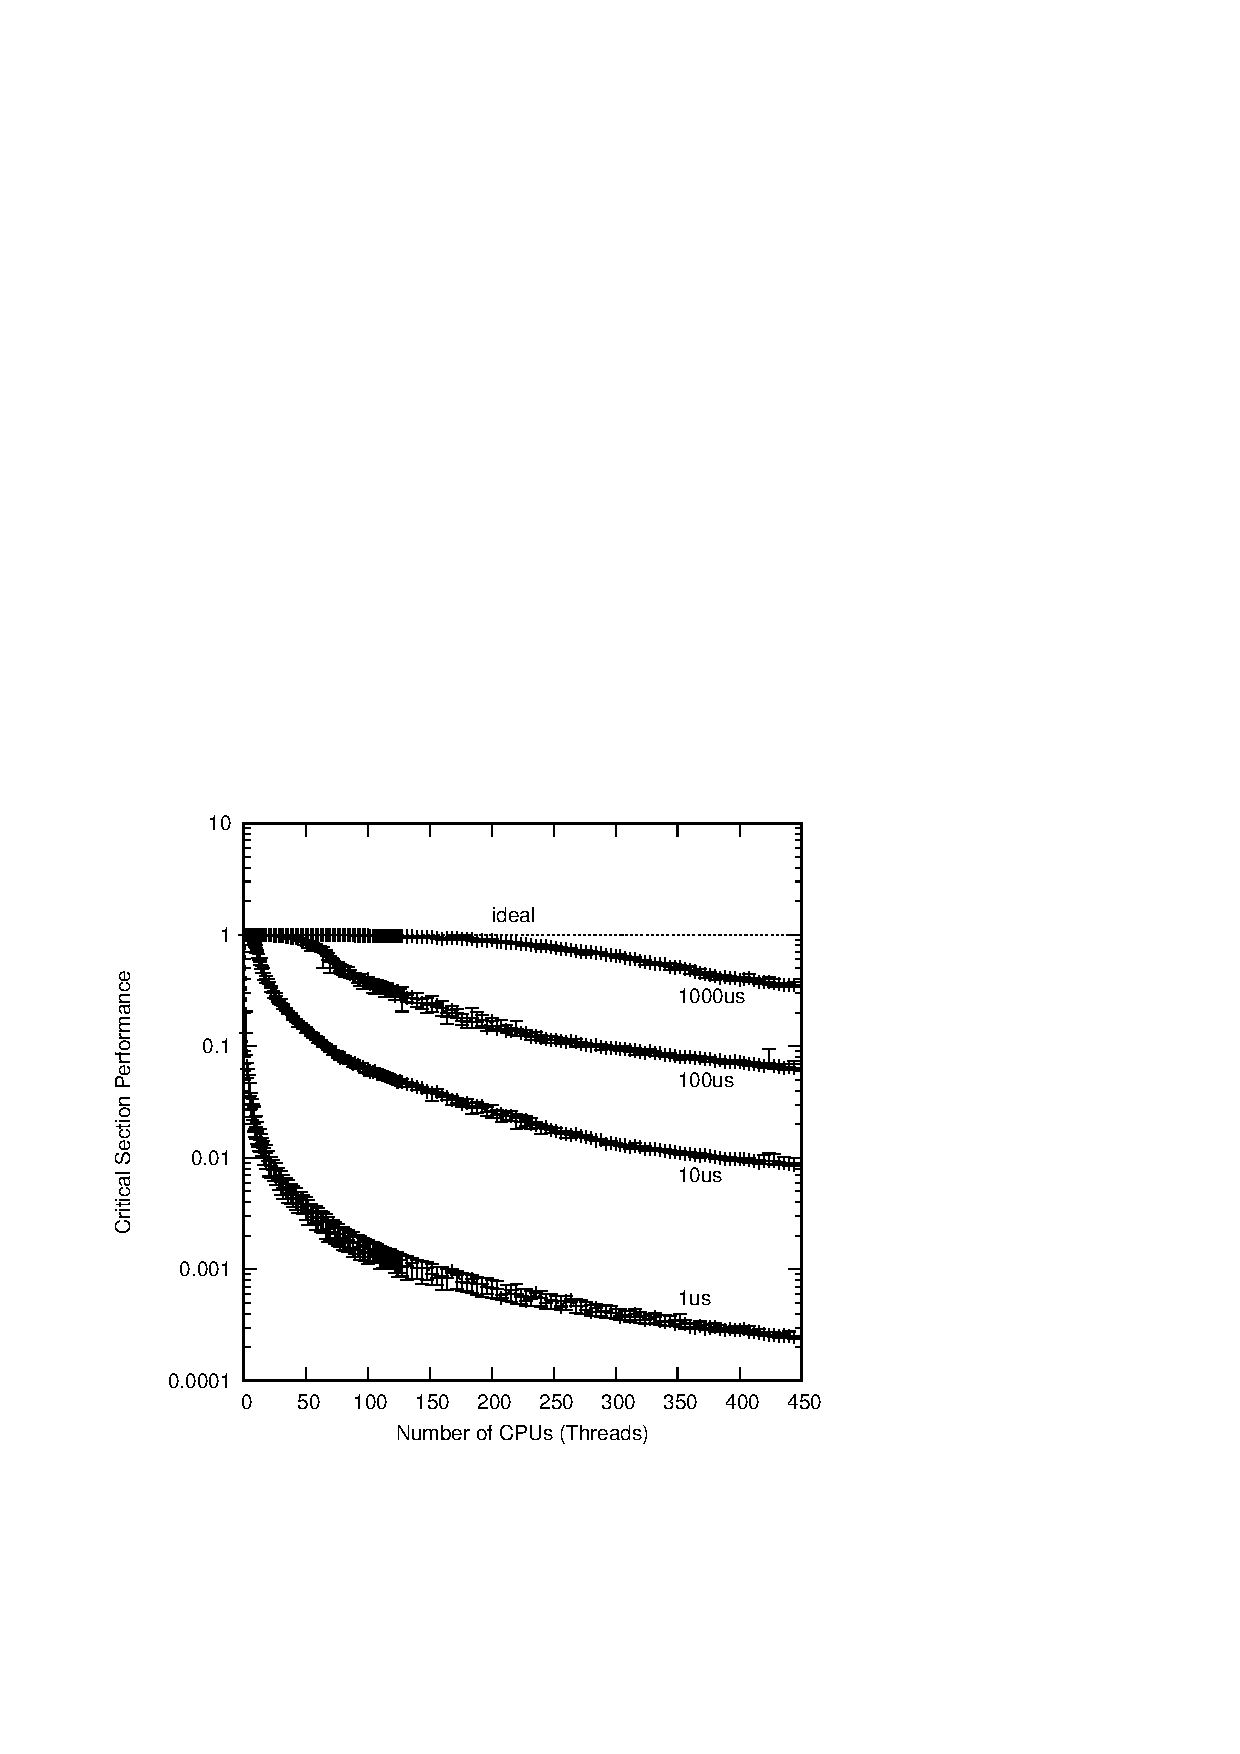
\includegraphics{CodeSamples/toolsoftrade/rwlockscale}}
\caption{Reader-Writer Lock Scalability}
\label{fig:intro:Reader-Writer Lock Scalability}
\end{figure}

Figure~\ref{fig:intro:Reader-Writer Lock Scalability}
shows the results of running this test on a 64-core Power-5 system
with two hardware threads per core for a total of 128 software-visible
CPUs.
The \co{thinktime} parameter was zero for all these tests, and the
\co{holdtime} parameter set to values ranging from one thousand (``1K''
on the graph) to 100 million (``100M'' on the graph).
The actual value plotted is:
\begin{equation}
	\frac{L_N}{N L_1}
\end{equation}
where $N$ is the number of threads,
$L_N$ is the number of lock acquisitions by $N$ threads, and
$L_1$ is the number of lock acquisitions by a single thread.
Given ideal hardware and software scalability, this value will always
be 1.0.

As can be seen in the figure, reader-writer locking scalability is
decidedly non-ideal, especially for smaller sizes of critical
sections.
To see why read-acquisition can be so slow, consider
that all the acquiring threads must update the \co{pthread_rwlock_t}
data structure.
Therefore, if all 128 executing threads attempt to
read-acquire the reader-writer lock concurrently, they must update
this underlying \co{pthread_rwlock_t} one at a time.
One lucky thread might do so almost immediately, but the least-lucky
thread must wait for all the other 127 threads to do their updates.
This situation will only get worse as you add CPUs.

\QuickQuiz{}
	Isn't comparing against single-CPU throughput a bit harsh?
\QuickQuizAnswer{
	Not at all.
	In fact, this comparison was, if anything, overly lenient.
	A more balanced comparison would be against single-CPU
	throughput with the locking primitives commented out.
} \QuickQuizEnd

\QuickQuiz{}
	But 1,000 instructions is not a particularly small size for
	a critical section.
	What do I do if I need a much smaller critical section, for
	example, one containing only a few tens of instructions?
\QuickQuizAnswer{
	If the data being read \emph{never} changes, then you do not
	need to hold any locks while accessing it.
	If the data changes sufficiently infrequently, you might be
	able to checkpoint execution, terminate all threads, change
	the data, then restart at the checkpoint.

	Another approach is to keep a single exclusive lock per
	thread, so that a thread read-acquires the larger aggregate
	reader-writer lock by acquiring its own lock, and write-acquires
	by acquiring all the per-thread locks~\cite{WilsonCHsieh92a}.
	This can work quite well for readers, but causes writers
	to incur increasingly large overheads as the number of threads
	increases.

	Some other ways of handling very small critical sections are
	described in Section~\ref{sec:defer:Read-Copy Update (RCU)}.
} \QuickQuizEnd

\QuickQuiz{}
	In
	Figure~\ref{fig:intro:Reader-Writer Lock Scalability},
	all of the traces other than the 100M trace deviate gently
	from the ideal line.
	In contrast, the 100M trace breaks sharply from the ideal
	line at 64 CPUs.
	In addition, the spacing between the 100M trace and the 10M
	trace is much smaller than that between the 10M trace and the
	1M trace.
	Why does the 100M trace behave so much differently than the
	other traces?
\QuickQuizAnswer{
	Your first clue is that 64 CPUs is exactly half of the 128
	CPUs on the machine.
	The difference is an artifact of hardware threading.
	This system has 64 cores with two hardware threads per core.
	As long as fewer than 64 threads are running, each can run
	in its own core.
	But as soon as there are more than 64 threads, some of the threads
	must share cores.
	Because the pair of threads in any given core share some hardware
	resources, the throughput of two threads sharing a core is not
	quite as high as that of two threads each in their own core.
	So the performance of the 100M trace is limited not by the
	reader-writer lock, but rather by the sharing of hardware resources
	between hardware threads in a single core.

	This can also be seen in the 10M trace, which deviates gently from
	the ideal line up to 64 threads, then breaks sharply down, parallel
	to the 100M trace.
	Up to 64 threads, the 10M trace is limited primarily by reader-writer
	lock scalability, and beyond that, also by sharing of hardware
	resources between hardware threads in a single core.
} \QuickQuizEnd

\QuickQuiz{}
	Power-5 is several years old, and new hardware should
	be faster.
	So why should anyone worry about reader-writer locks being slow?
\QuickQuizAnswer{
	In general, newer hardware is improving.
	However, it will need to improve more than two orders of magnitude
	to permit reader-writer lock to achieve ideal performance on
	128 CPUs.
	Worse yet, the greater the number of CPUs, the larger the
	required performance improvement.
	The performance problems of reader-writer locking are therefore
	very likely to be with us for quite some time to come.
} \QuickQuizEnd

Despite these limitations, reader-writer locking is quite useful in many
cases, for example when the readers must do high-latency file or network I/O.
There are alternatives, some of which will be presented in
Chapters~\ref{chp:Counting} and \ref{chp:Deferred Processing}.

\subsection{Atomic Operations (gcc Classic)}
\label{sec:toolsoftrade:Atomic Operations (gcc Classic)}

Given that
Figure~\ref{fig:intro:Reader-Writer Lock Scalability}
shows that the overhead of reader-writer locking is most severe for the
smallest critical sections, it would be nice to have some other way
to protect the tiniest of critical sections.
One such way are atomic operations.
We have seen one atomic operations already, in the form of the
\co{__sync_fetch_and_add()} primitive on line~18 of
Figure~\ref{fig:toolsoftrade:Measuring Reader-Writer Lock Scalability}.
This primitive atomically adds the value of its second argument to
the value referenced by its first argument, returning the old value
(which was ignored in this case).
If a pair of threads concurrently execute \co{__sync_fetch_and_add()} on
the same variable, the resulting value of the variable will include
the result of both additions.

The {\sf gcc} compiler offers a number of additional atomic operations,
including \co{__sync_fetch_and_sub()},
\co{__sync_fetch_and_or()},
\co{__sync_fetch_and_and()},
\co{__sync_fetch_and_xor()}, and
\co{__sync_fetch_and_nand()}, all of which return the old value.
If you instead need the new value, you can instead use the
\co{__sync_add_and_fetch()},
\co{__sync_sub_and_fetch()},
\co{__sync_or_and_fetch()},
\co{__sync_and_and_fetch()},
\co{__sync_xor_and_fetch()}, and
\co{__sync_nand_and_fetch()} primitives.

\QuickQuiz{}
	Is it really necessary to have both sets of primitives?
\QuickQuizAnswer{
	Strictly speaking, no.
	One could implement any member of the second set using the
	corresponding member of the first set.
	For example, one could implement \co{__sync_nand_and_fetch()}
	in terms of \co{__sync_fetch_and_nand()} as follows:

\vspace{5pt}
\begin{minipage}[t]{\columnwidth}
\scriptsize
\begin{verbatim}
tmp = v;
ret = __sync_fetch_and_nand(p, tmp);
ret = ~ret & tmp;
\end{verbatim}
\end{minipage}
\vspace{5pt}

	It is similarly possible to implement \co{__sync_fetch_and_add()},
	\co{__sync_fetch_and_sub()}, and \co{__sync_fetch_and_xor()}
	in terms of their post-value counterparts.

	However, the alternative forms can be quite convenient, both
	for the programmer and for the compiler/library implementor.
} \QuickQuizEnd

The classic compare-and-swap operation is provided by a pair of
primitives, \co{__sync_bool_compare_and_swap()} and
\co{__sync_val_compare_and_swap()}.
Both of these primitive atomically update a location to a new value,
but only if its prior value was equal to the specified old value.
The first variant returns 1 if the operation succeeded and 0 if it
failed, for example, if the prior value was not equal to the specified
old value.
The second variant returns the prior value of the location, which, if
equal to the specified old value, indicates that the operation succeeded.
Either of the compare-and-swap operation is ``universal'' in the sense
that any atomic operation on a single location can be implemented in
terms of compare-and-swap, though the earlier operations are often
more efficient where they apply.
The compare-and-swap operation is also capable of serving as the basis
for a wider set of atomic operations, though the more elaborate of
these often suffer from complexity, scalability, and performance
problems~\cite{MauriceHerlihy90a}.

The \co{__sync_synchronize()} primitive issues a ``memory barrier'',
which constrains both the compiler's and the CPU's ability to reorder
operations, as discussed in Section~\ref{sec:advsync:Memory Barriers}.
In some cases, it is sufficient to constrain the compiler's ability
to reorder operations, while allowing the CPU free rein, in which
case the \co{barrier()} primitive may be used, as it in fact was
on line~28 of
Figure~\ref{fig:toolsoftrade:Measuring Reader-Writer Lock Scalability}.
In some cases, it is only necessary to ensure that the compiler
avoids optimizing away a given memory access, in which case the
\co{ACCESS_ONCE()} primitive may be used, as it was on line~17 of
Figure~\ref{fig:toolsoftrade:Demonstration of Exclusive Locks}.
These last two primitives are not provided directly by gcc,
but may be implemented straightforwardly as follows:

\vspace{5pt}
{
\scriptsize
\begin{verbatim}
#define ACCESS_ONCE(x) (*(volatile typeof(x) *)&(x))
#define barrier() __asm__ __volatile__("": : :"memory")
\end{verbatim}
}
\vspace{5pt}

\QuickQuiz{}
	Given that these atomic operations will often be able to
	generate single atomic instructions that are directly
	supported by the underlying instruction set, shouldn't
	they be the fastest possible way to get things done?
\QuickQuizAnswer{
	Unfortunately, no.
	See Chapter~\ref{chp:Counting} for some stark counterexamples.
} \QuickQuizEnd

\subsection{Atomic Operations (C11)}
\label{sec:toolsoftrade:Atomic Operations (C11)}

The C11 standard added atomic operations,
including loads (\co{atomic_load()}),
stores (\co{atomic_store()}),
memory barriers (\co{atomic_thread_fence()} and
\co{atomic_signal_fence()}), and read-modified-write atomics.
The read-modify-write atomics include
\co{atomic_fetch_add()},
\co{atomic_fetch_sub()},
\co{atomic_fetch_and()},
\co{atomic_fetch_xor()},
\co{atomic_exchange()},
\co{atomic_compare_exchange_strong()},
and
\co{atomic_compare_exchange_weak()}.
These operate in a manner similar to those described in
Section~\ref{sec:toolsoftrade:Atomic Operations (gcc Classic)},
but with the addition of memory-order arguments to \co{_explicit}
variants of all of the operations.
Without memory-order arguments, all the atomic operations are
fully ordered, and the arguments permit weaker orderings.
For example, ``\co{memory_order_explicit(&a, memory_order_relaxed)}''
is vaguely similar to the Linux kernel's ``\co{READ_ONCE()}''.\footnote{
	Memory ordering is described in more detail in
	Section~\ref{sec:advsync:Memory Barriers} and
	Appendix~\ref{chp:app:whymb:Why Memory Barriers?}.}

One restriction of the C11 atomics is that they apply only to special
atomic types, which can be restrictive.
The gcc compiler therefore provides
\co{__atomic_load()},
\co{__atomic_load_n()},
\co{__atomic_store()},
\co{__atomic_store_n()}, etc.
These primitives offer the same semantics as their C11 counterparts,
but may be used on plain non-atomic objects.

\section{Linux-Kernel Equivalents to POSIX Operations}
\label{sec:toolsoftrade:Linux-Kernel Equivalents to POSIX Operations}

\begin{table*}
\scriptsize
\centering
\begin{tabular}{l|l|l}
	Category & POSIX & Linux Kernel \\
	\hline
	\hline
	Thread Management
		& \co{pthread_t}
			& \co{struct task_struct} \\
	\cline{2-3}
		& \co{pthread_create()}
			& \co{kthread_create} \\
	\cline{2-3}
		& \co{pthread_exit()}
			& \co{kthread_should_stop()}~~~~~(rough) \\
	\cline{2-3}
		& \co{pthread_join()}
			& \co{kthread_stop()}~~~(rough) \\
	\cline{2-3}
		& \co{poll(NULL, 0, 5)}
			& \co{schedule_timeout_interruptible()} ~~~ \\
	\hline
	\hline
	POSIX Locking
		& \co{pthread_mutex_t}
			& \co{spinlock_t}~~~(rough) \\
		&	& \co{struct mutex} \\
	\cline{2-3}
		& \co{PTHREAD_MUTEX_INITIALIZER}
			& \co{DEFINE_SPINLOCK()} \\
		&	& \co{DEFINE_MUTEX()} \\
	\cline{2-3}
		& \co{pthread_mutex_lock()}
			& \co{spin_lock()}~~~(and friends) \\
		&	& \co{mutex_lock()}~~~(and friends) \\
	\cline{2-3}
		& \co{pthread_mutex_unlock()}
			& \co{spin_unlock()}~~~(and friends) \\
		&	& \co{mutex_unlock()} \\
	\hline
	\hline
	POSIX Reader-Writer
		& \co{pthread_rwlock_t}
			& \co{rwlock_t}~~~(rough) \\
	Locking	&	& \co{struct rw_semaphore} \\
	\cline{2-3}
		& \co{PTHREAD_RWLOCK_INITIALIZER}
			& \co{DEFINE_RWLOCK()} \\
		&	& \co{DECLARE_RWSEM()} \\
	\cline{2-3}
		& \co{pthread_rwlock_rdlock()}
			& \co{read_lock()}~~~(and friends) \\
		&	& \co{down_read()}~~~(and friends) \\
	\cline{2-3}
		& \co{pthread_rwlock_unlock()}
			& \co{read_unlock()}~~~(and friends) \\
		&	& \co{up_read()} \\
	\cline{2-3}
		& \co{pthread_rwlock_wrlock()}
			& \co{write_lock()}~~~(and friends) \\
		&	& \co{down_write()}~~~(and friends) \\
	\cline{2-3}
		& \co{pthread_rwlock_unlock()}
			& \co{write_unlock()}~~~(and friends) \\
		&	& \co{up_write()} \\
	\hline
	\hline
	Atomic Operations
		& C Scalar Types
			& \co{atomic_t} \\
		&	& \co{atomic64_t} \\
	\cline{2-3}
		& \co{__sync_fetch_and_add()}
			& \co{atomic_add_return()} \\
		&	& \co{atomic64_add_return()} \\
	\cline{2-3}
		& \co{__sync_fetch_and_sub()}
			& \co{atomic_sub_return()} \\
		&	& \co{atomic64_sub_return()} \\
	\cline{2-3}
		& \co{__sync_val_compare_and_swap()} ~~~~~~~~~~
			& \co{cmpxchg()} \\
	\cline{2-3}
		& \co{__sync_lock_test_and_set()}
			& \co{xchg()}~~~(rough) \\
	\cline{2-3}
		& \co{__sync_synchronize()}
			& \co{smp_mb()} \\
\end{tabular}
\caption{Mapping from POSIX to Linux-Kernel Primitives}
\label{tab:advsync:Mapping from POSIX to Linux-Kernel Primitives}
\end{table*}

Unfortunately, threading operations, locking primitives, and atomic
operations were in reasonably wide use long before the various standards
committees got around to them.
As a result, there is considerable variation in how these operations
are supported.
It is still quite common to find these operations implemented in
assembly language, either for historical reasons or to obtain better
performance in specialized circumstances.
For example, the gcc \co{__sync_} family of primitives all
provide memory-ordering semantics, motivating many developers to
create their own implementations for situations where the memory
ordering semantics are not required.

Therefore,
Table~\ref{tab:advsync:Mapping from POSIX to Linux-Kernel Primitives} on
page~\pageref{tab:advsync:Mapping from POSIX to Linux-Kernel Primitives}
provides a rough mapping between the POSIX and
gcc primitives to those used in the Linux kernel.
Exact mappings are not always available, for example, the Linux kernel
has a wide variety of locking primitives, while gcc has a number
of atomic operations that are not directly available in the Linux kernel.
Of course, on the one hand, user-level code does not need the Linux
kernel's wide array of locking primitives, while on the other hand,
gcc's atomic operations can be emulated reasonably straightforwardly
using \co{cmpxchg()}.

\QuickQuiz{}
	What happened to the Linux-kernel equivalents to \co{fork()}
	and \co{wait()}?
\QuickQuizAnswer{
	They don't really exist.
	All tasks executing within the Linux kernel share memory,
	at least unless you want to do a huge amount of memory-mapping
	work by hand.
} \QuickQuizEnd

\section{The Right Tool for the Job: How to Choose?}
\label{sec:toolsoftrade:The Right Tool for the Job: How to Choose?}

As a rough rule of thumb, use the simplest tool that will get the job done.
If you can, simply program sequentially.
If that is insufficient, try using a shell script to mediate parallelism.
If the resulting shell-script \co{fork()}/\co{exec()} overhead
(about 480 microseconds for a minimal C program on an Intel Core Duo
laptop) is too
large, try using the C-language \co{fork()} and \co{wait()} primitives.
If the overhead of these primitives (about 80 microseconds for a minimal
child process) is still too large, then you
might need to use the POSIX threading primitives, choosing the appropriate
locking and/or atomic-operation primitives.
If the overhead of the POSIX threading primitives (typically sub-microsecond)
is too great, then the primitives introduced in
Chapter~\ref{chp:Deferred Processing} may be required.
Always remember that inter-process communication and message-passing
can be good alternatives to shared-memory multithreaded execution.

\QuickQuiz{}
	Wouldn't the shell normally use \co{vfork()} rather than
	\co{fork()}?
\QuickQuizAnswer{
	It might well do that, however, checking is left as an exercise
	for the reader.
	But in the meantime, I hope that we can agree that \co{vfork()}
	is a variant of \co{fork()}, so that we can use \co{fork()}
	as a generic term covering both.
} \QuickQuizEnd

Of course, the actual overheads will depend not only on your hardware,
but most critically on the manner in which you use the primitives.
In particular, randomly hacking multi-threaded code is a spectacularly
bad idea, especially given that shared-memory parallel systems use
your own intelligence against you:
The smarter you are, the deeper a hole you will dig for yourself before
you realize that you are in trouble~\cite{DeadlockEmpire2016}.
Therefore, it is necessary to make the right design choices as well as
the correct choice of individual primitives,
as is discussed at length in subsequent chapters.
